\section{Performance analysis}

The questionnaires show lower self-reported \ac{uml} competence in the \ac{pv} variant before taking the course. Self-reported competence equalizes after the students have completed the courses. 

\FloatBarrier
\begin{figure}[ht]
\centering
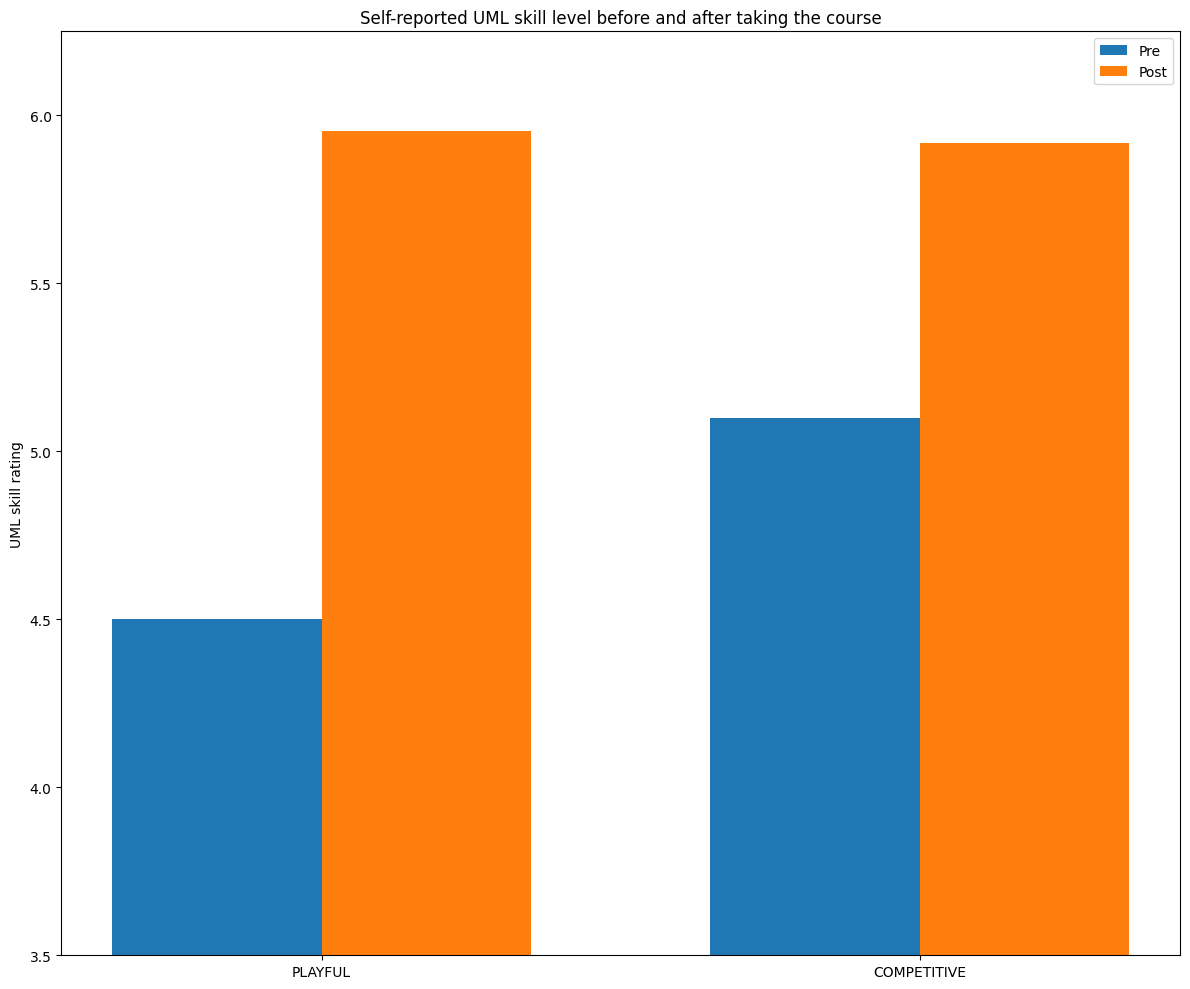
\includegraphics[width=0.6\textwidth]{assets/images/eval/uml_self_reported_skill_plot.png}
\caption{Self-reported skill in \ac{uml} before and after taking the course}
\label{fig:uml_self_reported_skill_plot}
\end{figure}
\FloatBarrier

Despite the self-reported competence equalizing, the variance of the metric decreased in the \ac{pv}, and increased in the \ac{cv}. That indicates the \ac{cv} might have polarizing effects on the learners' perception.

\FloatBarrier
\begin{table}[h]
\centering
\renewcommand{\arraystretch}{1.2}
\begin{tabular}{l l c c c}
\hline
\textbf{Group} & \textbf{Phase} & \textbf{Mean} & \textbf{Median} & \textbf{Variance} \\
\hline
Playful      & Introduction    & 4.50 & 4.0 & 5.91 \\
Playful      & Feedback & 5.95 & 6.0 & 5.15 \\
Competitive  & Introduction    & 5.10 & 5.0 & 2.73 \\
Competitive  & Feedback & 5.92 & 6.5 & 5.72 \\
\hline
\end{tabular}
\caption{Self-reported UML skill ratings across course variants before (Introduction) and after (Feedback) the intervention.}
\label{tab:uml_skill_comparison}
\end{table}
\FloatBarrier

The \ac{pv} exhibits higher improvement rates among participants. The difference in improvement is not statistically significant (Mann–Whitney U, p=0.21279), a moderate effect size is observed (Cohen’s d=0.472).

The Intro score is also lower in \ac{pv}, while Final score is roughly equal in both variants. Along with a significant decrease in variance and standard deviation between Intro score and Final score in \ac{pv}, we can infer there is a ceiling to performance to which both groups converged. We should take note of students in \ac{pv} starting with more diverse levels of skill.

\FloatBarrier
\begin{table}[h]
\centering
\renewcommand{\arraystretch}{1.2}
\begin{tabular}{l l c c c c c}
\hline
\textbf{Group} & \textbf{Metric} & \textbf{Mean} & \textbf{Median} & \textbf{Variance} & \textbf{Std} \\
\hline
C & Improvement  & 1.47 & 2.48 & 113.95 & 10.67 \\
C & Intro score  & 85.55 & 83.59 & 108.01 & 10.39 \\
C & Final score  & 87.02 & 88.53 & 82.34  & 9.07 \\
P & Improvement  & 6.81 & 6.12 & 137.68 & 11.73 \\
P & Intro score  & 78.55 & 82.37 & 225.24 & 15.01 \\
P & Final score  & 85.35 & 87.33 & 132.40 & 11.51 \\
\hline
\end{tabular}
\caption{Descriptive statistics of performance metrics for competitive (C) and playful (P) course variants.}
\label{tab:desc_stats_cp}
\end{table}
\FloatBarrier

We can see that students with lower Intro scores tended to improve more significantly, while high-scoring individuals even worsened in some cases.

\FloatBarrier
\begin{figure}[ht]
\centering
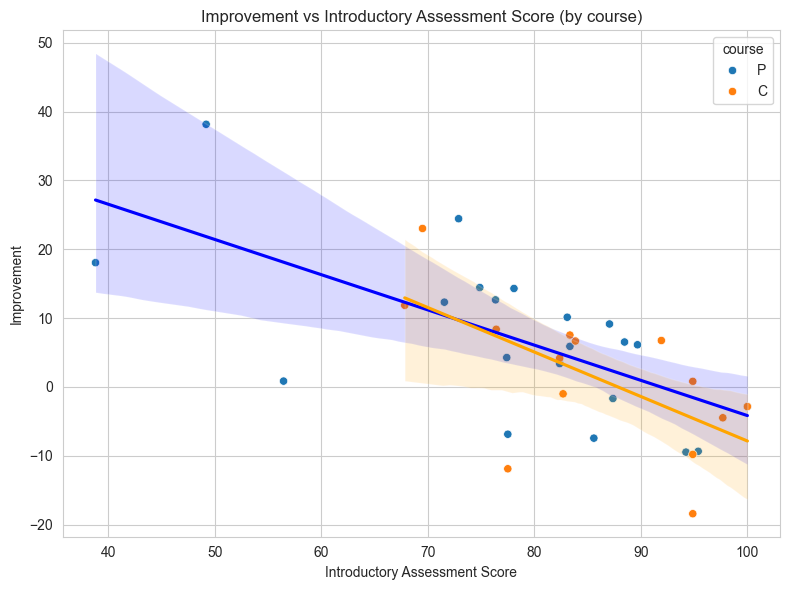
\includegraphics[width=0.6\textwidth]{assets/images/eval/imporvement_vs_introductory_assessment_score.png}
\caption{Improvement vs score in the introductory assessment quiz}
\label{fig:imporvement_vs_introductory_assessment_score}
\end{figure}
\FloatBarrier


% In the following table, we can see average score across all exercises and the standard deviation of the scores, grouped by course variant. Again, the \ac{pv} has lower average score and a higher standard deviation in the scores, which is in line with an overall lower as well as more diverse starting point for the variant.

% \FloatBarrier
% \begin{table}[h]
% \centering
% \renewcommand{\arraystretch}{1.2}
% \begin{tabular}{l c c c c c}
% \hline
% \textbf{Metric} & \textbf{Avg. Score (C)} & \textbf{Std (C)} & \textbf{Avg. Score (P)} & \textbf{Std (P)} & \textbf{Diff} \\
% \hline

% Mean     & 82.74 & 16.57 & 77.89 & 19.85 &  4.85 \\
% Median   & 89.79 & 12.81 & 86.10 & 18.19 &  2.79 \\
% Variance & 403.44 & 98.15 & 506.08 & 81.06 & 48.18 \\
% Std Dev  & 20.09 &  9.91 & 22.50 &  9.00 &  6.94 \\

% \hline
% \end{tabular}
% \caption{Descriptive statistics of exercise performance for competitive (C) and playful (P) variants.}
% \label{tab:exercise_stats_comparison}
% \end{table}
% \FloatBarrier

The last figure shows performance across exercise categories. \ac{cv} scores consistently higher in all categories except for one. 
% The average difference between the variants is 4.34, which roughly corresponds to the higher baseline skill level in \ac{pv}.

When comparing performance in individual exercises, \ac{pv} only scores better in 5 out of 28. That is a noticeable difference, which might not be attributed to a slightly higher baseline knowledge alone.

\FloatBarrier
\begin{figure}[ht]
\centering
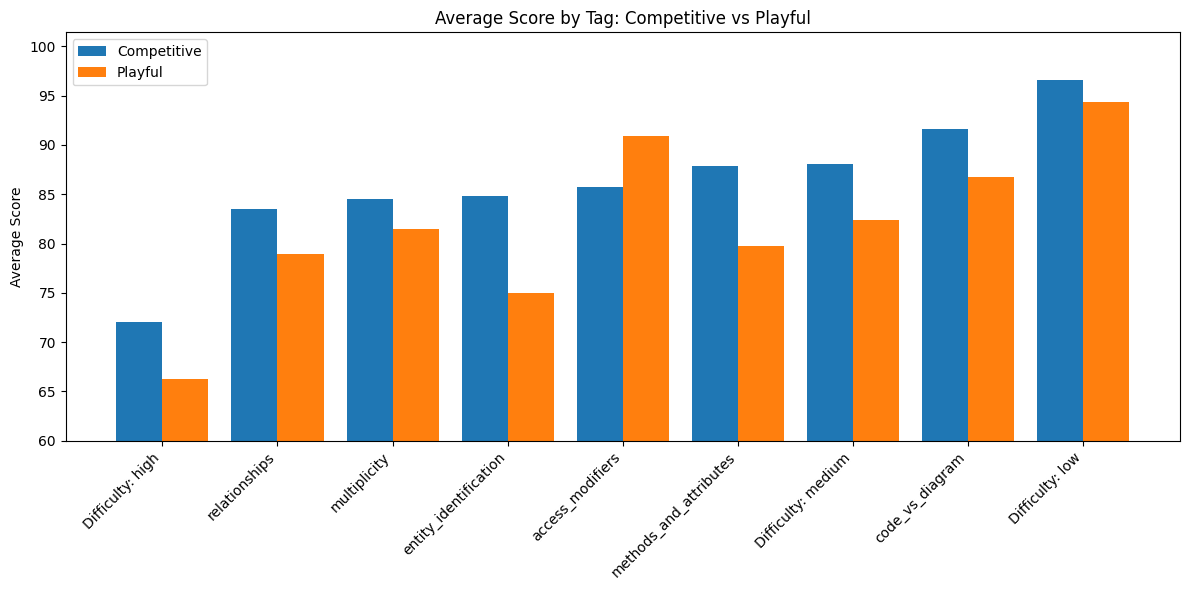
\includegraphics[width=1\textwidth]{assets/images/eval/avg_score_by_tag.png}
\caption{Average score by tag for Competitive and Playful variants}
\label{fig:avg_score_by_tag}
\end{figure}
\FloatBarrier


% \todo{summary? Maybe?}
% \textbf{Summary}

% The objective performance is higher in \ac{cv}, while improvement rates are higher in \ac{pv}. This can be explained mainly by the fact that \ac{cv} has a higher baseline skill, which also reduces the potential for improvement in its participants. However, the results show very consistently higher scores across all activities in \ac{cv}, which might not be caused by the skill difference alone.

